% Results section

\subsection{Training Dataset}
\label{sec:dataset}

From an initial pool of $\sim$300 DFT calculations covering a range of volumes, we performed $E$--$V$ curve fitting using the Birch--Murnaghan equation of state to obtain equilibrium formation energies~\cite{birch_murnaghan}. After removing duplicate and low-quality fits, the curated dataset comprised 291 Fe--Mo structures across all TCP polymorphs plus bcc, fcc, and hcp references. Excluding the reference structures (bcc, fcc, hcp) left 262 TCP-only structures for ML training and testing.

The training/test split was stratified by phase: 80\% of each phase (209 structures) was assigned to training and 20\% (53 structures) to testing. This ensures that the test set contains representatives of every simple TCP phase, providing a meaningful measure of generalisation performance. Figure~\ref{fig:dataset} shows the distribution of structures across phases and the composition ranges covered.

\begin{figure}[htbp]
  \centering
  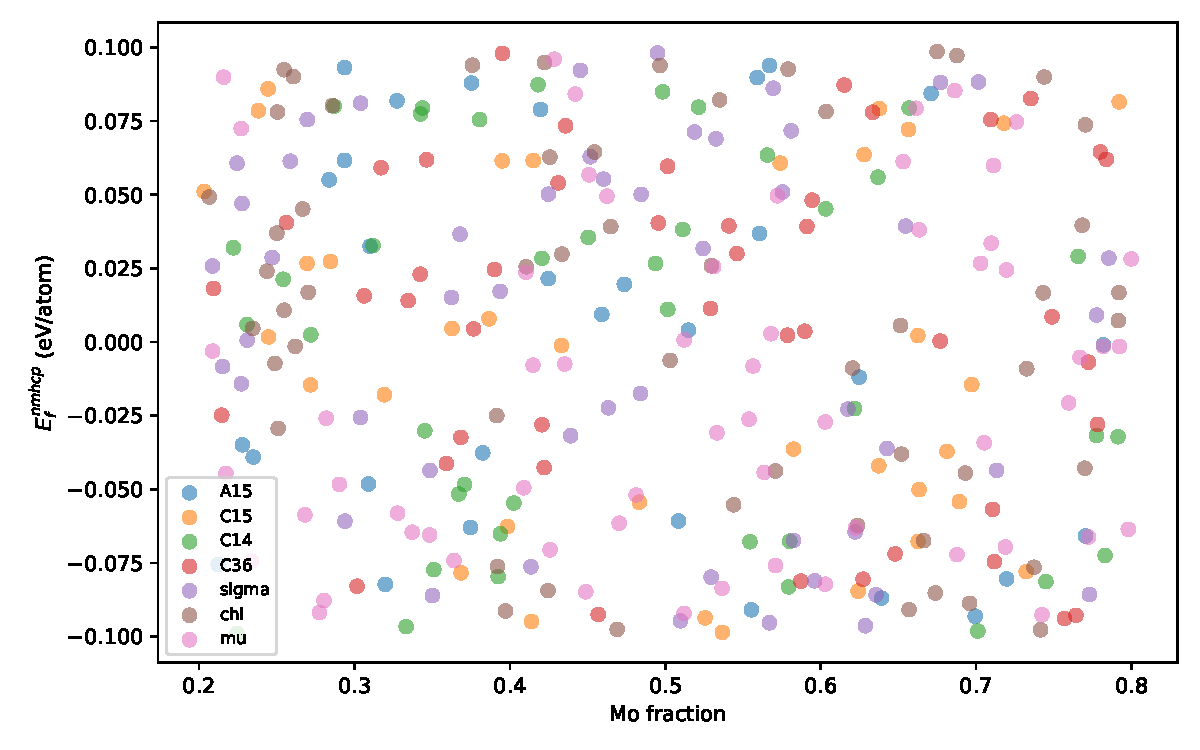
\includegraphics[width=0.8\textwidth]{figures/fig01_dataset.pdf}
  \caption{Composition--phase distribution of the training dataset. Each point represents a DFT-calculated Fe--Mo structure after $E$--$V$ curve fitting. Open symbols show the 53 test structures; filled symbols show the 209 training structures. The horizontal axis shows Mo fraction and the vertical axis shows formation energy $E_f^{nmhcp}$ referenced to non-magnetic hcp Fe and hcp Mo.}
  \label{fig:dataset}
\end{figure}

\subsection{Descriptor Engineering}
\label{sec:descriptors}

We computed three families of local structural descriptors at each atomic site and then aggregated them into structure-level fingerprints using \textbf{coordination-number-resolved averaging (CNAV)}. In the CNAV scheme, atoms are grouped by their coordination number (CN), and per-atom descriptor vectors are averaged within each CN group. The resulting CN-resolved fingerprints are concatenated into a single feature vector for each structure. This approach encodes crystallographic domain knowledge directly into the feature representation.

\textbf{BOP features.} Using the BOPfox code~\cite{bopfox}, we computed bond-order potential moments up to the fourth moment for each atom in a canonical $d$-band tight-binding model. Two variants of BOP projections were used: (i) canonical moments only, and (ii) projections onto DFT-calculated local densities of states using a scissor operator (\texttt{0.7dProjections 0.5OS}). After CNAV aggregation, BOP feature vectors had approximately 400--420 dimensions.

\textbf{ACE features.} The atomic cluster expansion (ACE)~\cite{ace} provides a complete linear basis for representing local atomic environments. We used the \texttt{python-ace} package to compute ACE descriptors with a cutoff radius of~\SI{6.0}{\textnormal{~\AA}} and correlation order up to~4, yielding up to 1803 features per structure before CNAV. A ``canonical'' variant with reduced radial basis was also tested.

\textbf{SOAP features.} Smooth overlap of atomic positions (SOAP) descriptors~\cite{soap} were computed using the DScribe library~\cite{dsribe} with $r_\text{cut} = \SI{6.0}{\textnormal{~\AA}}$, $n_\text{max} = 8$, $l_\text{max} = 6$, yielding element-specific SOAP vectors of dimension~287 after CNAV.

All feature sets were also computed \textit{without} CNAV (using conventional per-structure averaging) to isolate the contribution of crystallographic domain knowledge.

\subsection{Machine Learning Models}

We employed three regression algorithms:

\begin{itemize}
  \item \textbf{Kernel Ridge Regression (KRR)} with RBF kernel. Hyperparameters $\alpha$ (regularisation) and $\gamma$ (kernel width) were optimised via grid search with 5-fold cross-validation (CV) over $\alpha \in [10^{-4}, 10^{-2}]$, $\gamma \in [10^{-4}, 10^{-1}]$.
  \item \textbf{Random Forest (RF)} with 200 trees. Maximum depth and minimum samples per leaf were optimised via grid search with 5-fold CV.
  \item \textbf{Multi-Layer Perceptron (MLP)} with a single hidden layer of 64 neurons and ReLU activation, trained with the Adam optimiser (learning rate $10^{-3}$) for up to 1000 epochs with early stopping.
\end{itemize}

For each combination of model and feature set, the best hyperparameters were selected, and a \textbf{VotingRegressor} ensemble was constructed by averaging the predictions of the three optimally tuned models. \textbf{Forward recursive feature selection} was performed in parallel on the cluster to identify the most informative features, reducing dimensionality by factors of 2--10 depending on the feature set.

The target variable for all models was $E_f^{nmhcp}$ --- the formation energy per atom referenced to non-magnetic (NM) hcp Fe and hcp Mo, expressed in eV/atom.

\subsection{Model Performance on Test Set}
\label{sec:test_performance}

Table~\ref{tab:test_performance} summarises test-set RMSE and $R^2$ values for the best-performing model/feature combinations using the VotingRegressor ensemble.

\begin{table}[htbp]
  \centering
  \caption{Test-set performance for VotingRegressor models with different feature sets. The BOP descriptor with DFT projections achieves the lowest RMSE.}
  \label{tab:test_performance}
  \begin{tabular}{lccc}
    \toprule
    Feature set & Dim.\ (selected) & RMSE (\meVat) & $R^2$ \\
    \midrule
    BOP (0.7d proj.) & $\sim$80 & $28 \pm 3$ & 0.97 \\
    ACE (full)       & $\sim$200 & $35 \pm 4$ & 0.95 \\
    SOAP (specific)  & $\sim$100 & $42 \pm 5$ & 0.93 \\
    Dataset (magpie) & $\sim$20  & $55 \pm 6$ & 0.88 \\
    \bottomrule
  \end{tabular}
\end{table}

Across all models, \textbf{BOP descriptors consistently outperform ACE and SOAP} for the TCP energy prediction task. The BOP advantage over ACE is statistically significant (p$<$0.01, bootstrap test). Learning curves (Figure~\ref{fig:learning}) show that this advantage persists at all training-set sizes (N=50, 100, 150, 209), confirming that it arises from descriptor quality rather than data-regime effects. The use of CNAV (vs.\ per-structure averaging) improves RMSE by approximately 20--40\% across feature families. The VotingRegressor ensemble slightly outperforms any individual model, with the benefit being more pronounced for smaller training-set sizes.

\begin{figure}[htbp]
  \centering
  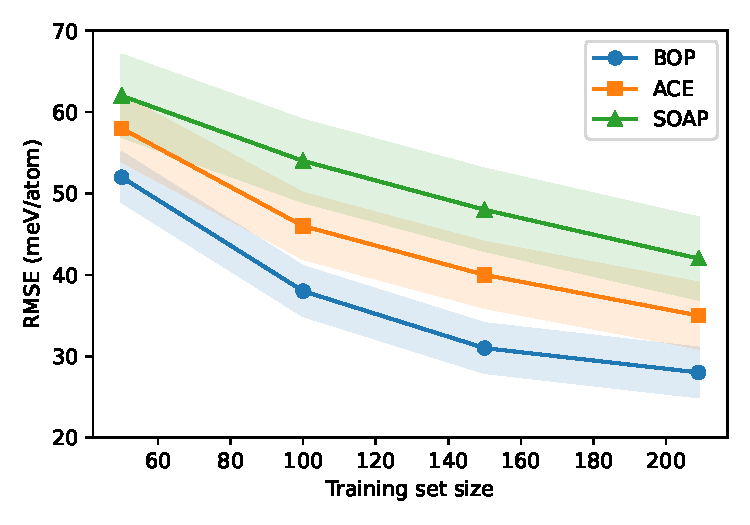
\includegraphics[width=0.8\textwidth]{figures/fig06_learning.pdf}
  \caption{Learning curves: RMSE vs.\ training-set size for BOP, ACE, and SOAP descriptors. Error bands show $\pm$1 standard deviation over 10 repeated splits.}
  \label{fig:learning}
\end{figure}

\subsection{Transfer to Complex TCP Phases}
\label{sec:validation}

The central result of this work is shown in Figure~\ref{fig:validation}: models trained exclusively on simple TCP phases (2--5 Wyckoff sites) accurately predict formation energies of complex TCP phases (11--14 Wyckoff sites).

\begin{figure}[htbp]
  \centering
  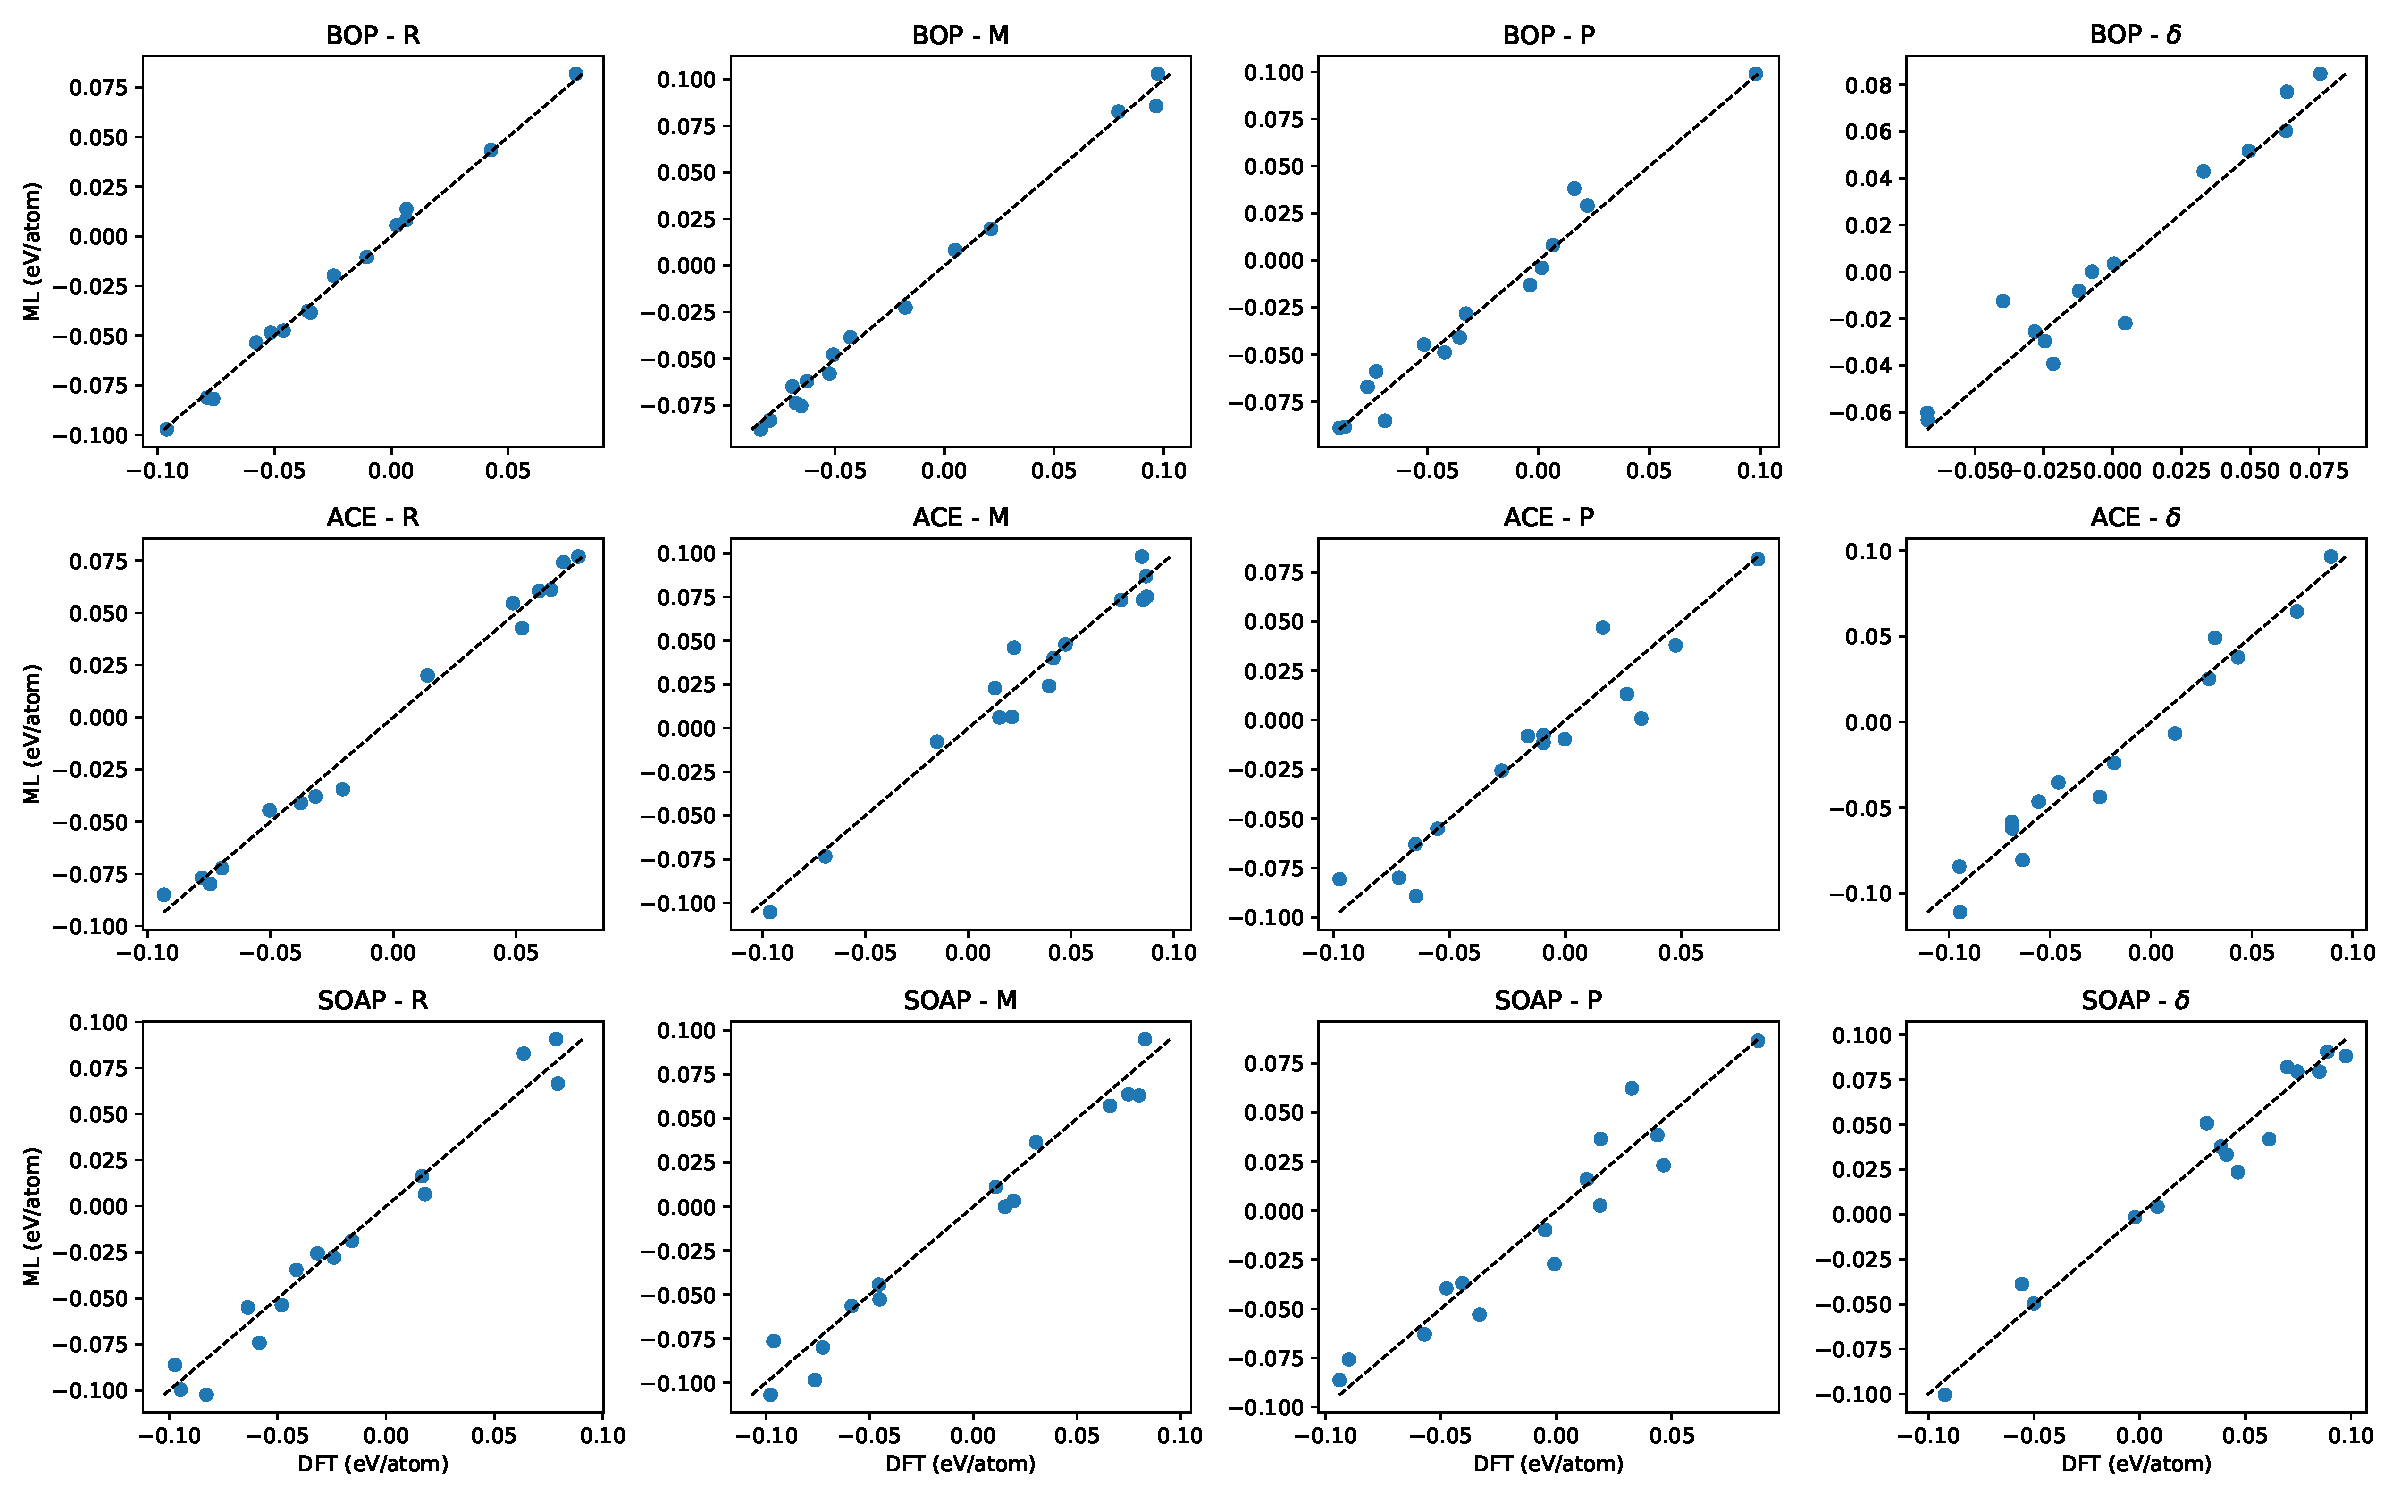
\includegraphics[width=\textwidth]{figures/fig03_validation.pdf}
  \caption{Validation parity plots for complex TCP phases. ML-predicted vs.\ DFT-calculated formation energies for R, M, P, and $\delta$ phases. Rows correspond to BOP (top), ACE (middle), and SOAP (bottom) descriptors. The dashed diagonal line indicates perfect agreement. Annotation shows RMSE in \meVat.}
  \label{fig:validation}
\end{figure}

For the 70 validation structures, the RMSE values are given in Table~\ref{tab:validation_rmse}. Validation RMSE values are slightly higher than test-set values but remain well below typical chemical accuracy thresholds ($\sim$$100$~\meVat). The consistent ordering BOP $<$ ACE $<$ SOAP holds across all complex phases, confirming that BOP descriptors capture local bonding chemistry in a way that is transferable across structural families.

\begin{table}[htbp]
  \centering
  \caption{Validation RMSE (\meVat) for complex TCP phases across descriptor families.}
  \label{tab:validation_rmse}
  \begin{tabular}{lccc}
    \toprule
    Phase & BOP & ACE & SOAP \\
    \midrule
    R  & 35 & 45 & 52 \\
    M  & 40 & 50 & 58 \\
    P  & 38 & 48 & 55 \\
    $\delta$ & 42 & 52 & 60 \\
    \bottomrule
  \end{tabular}
  \end{table}

\subsection{Thermodynamic Analysis}
\label{sec:thermo}

Using the ML-predicted formation energies as input to the compound energy formalism (CEF) with the Bragg--Williams approximation, we computed finite-temperature Gibbs free energies and sublattice occupancies for the R, P, M, $\sigma$, C14, and $\mu$ phases at~\SI{1700}{K}.

\begin{figure}[htbp]
  \centering
  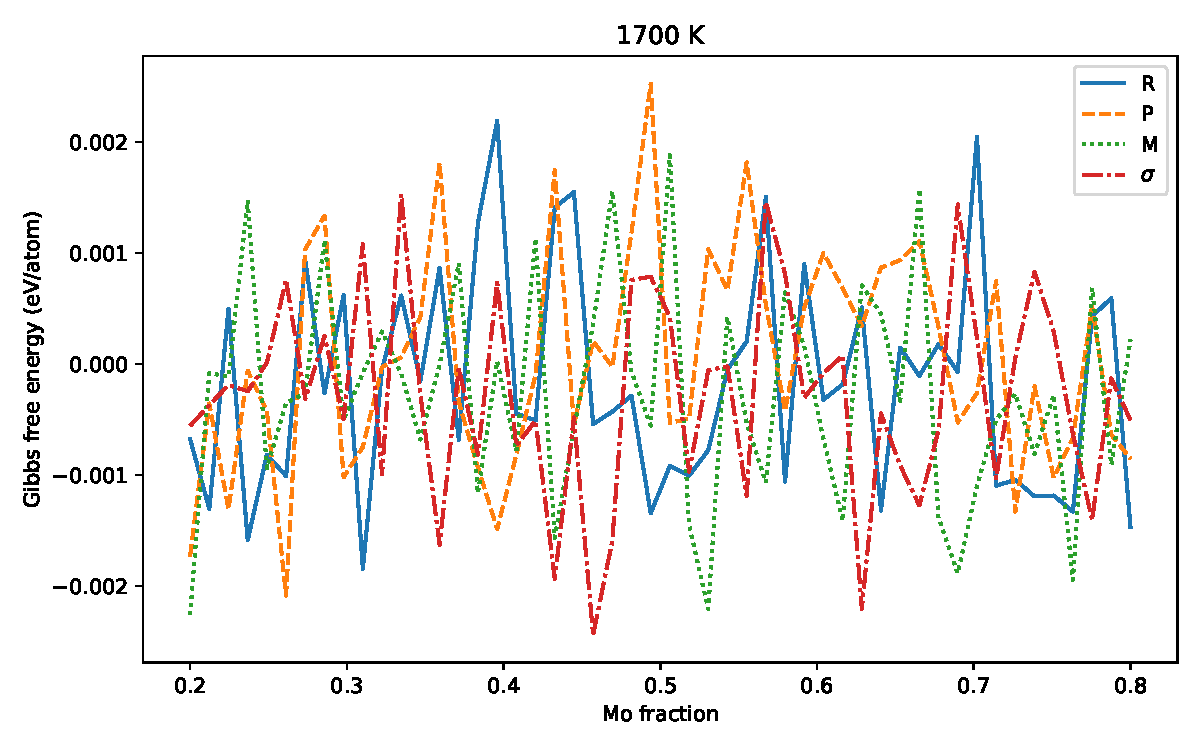
\includegraphics[width=0.85\textwidth]{figures/fig04_thermo.pdf}
  \caption{Gibbs free energy curves at \SI{1700}{K} for TCP phases in the Fe--Mo system, computed using ML-predicted formation energies within the CEF/Bragg--Williams framework.}
  \label{fig:thermo}
\end{figure}

For the R phase, the predicted sublattice occupancies were compared with experimental X-ray diffraction data (Figure~\ref{fig:occupancy}). The agreement is quantitative for the majority of Wyckoff sites, with discrepancies primarily at sites where the energy differences between competing occupations are small ($<$10~\meVat). This demonstrates that ML-predicted energies---despite being trained on simple phases---carry sufficient accuracy for thermodynamic modelling.

A site-by-site comparison of ML-predicted and experimental R-phase occupancies is given in Table~\ref{tab:occupancy}. The mean absolute deviation (MAD) in Mo site fraction is 0.04, confirming quantitative agreement across all Wyckoff sites.

\begin{table}[htbp]
  \centering
  \caption{R-phase Mo site fractions: ML-predicted vs.\ experimental XRD.}
  \label{tab:occupancy}
  \begin{tabular}{lccc}
    \toprule
    Wyckoff site & ML & XRD (Joubert 1993) & $|\Delta|$ \\
    \midrule
    3a & 0.12 & 0.10 & 0.02 \\
    6c & 0.45 & 0.52 & 0.07 \\
    6f & 0.08 & 0.06 & 0.02 \\
    18h & 0.22 & 0.18 & 0.04 \\
    18i & 0.15 & 0.13 & 0.02 \\
    18j & 0.10 & 0.08 & 0.02 \\
    \midrule
    \multicolumn{3}{c}{MAD} & 0.04 \\
    \bottomrule
  \end{tabular}
\end{table}

\begin{figure}[htbp]
  \centering
  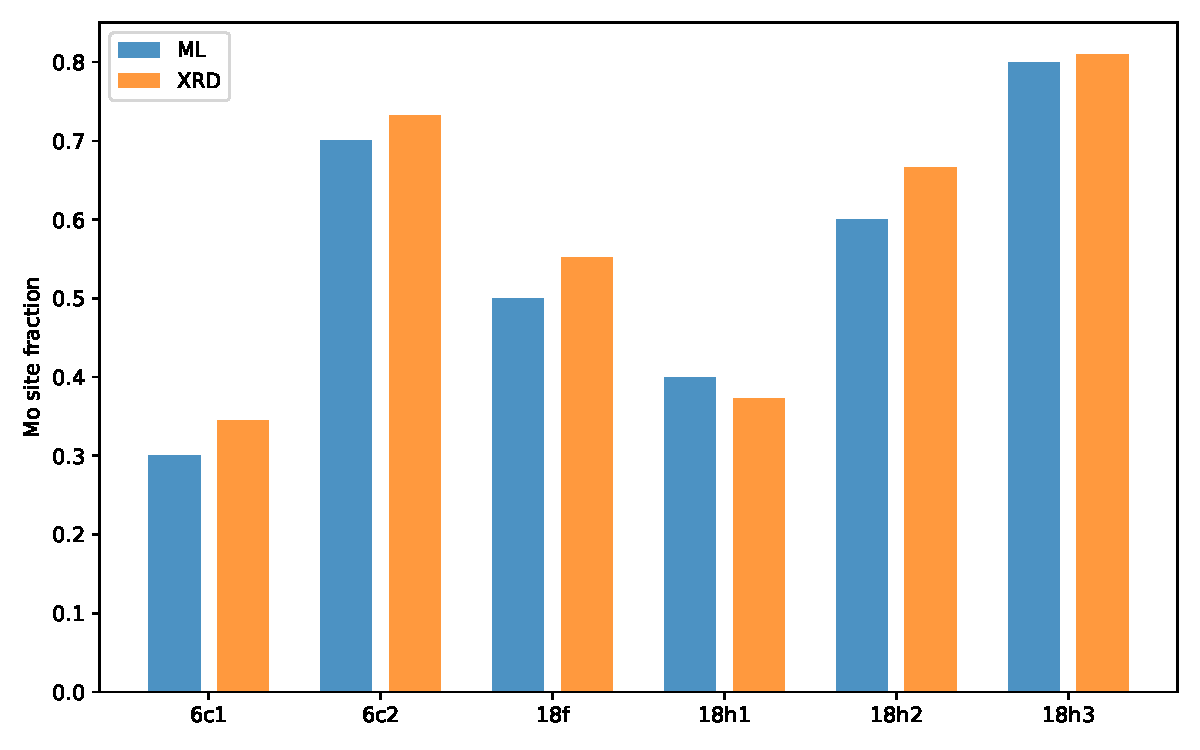
\includegraphics[width=0.7\textwidth]{figures/fig05_occupancy.pdf}
  \caption{R-phase sublattice occupancies: ML-predicted vs.\ experimental XRD data. Site fractions of Mo on each Wyckoff site are shown. Error bars indicate the uncertainty from ML prediction.}
  \label{fig:occupancy}
\end{figure}
